\documentclass[10pt]{article}
\usepackage[utf8]{inputenc}
\usepackage[spanish]{babel}
\usepackage{amsmath}
\usepackage{amsfonts}
\usepackage{amssymb}
\usepackage{graphics}
\usepackage{graphicx}
\usepackage[left=2cm,right=2cm,top=2cm,bottom=2cm]{geometry}
\usepackage{imakeidx}
\makeindex[columns=3, title=Alphabetical Index, intoc]
\usepackage{listings}
\usepackage{multicol}
\usepackage{changepage}
\usepackage{float}
\usepackage{cite}
\usepackage{url}
\usepackage{hyperref}
\usepackage{pdflscape}
\usepackage[document]{ragged2e}
\usepackage{xcolor,colortbl}

\hypersetup{
    colorlinks=true,
    linkcolor=blue,
    filecolor=magenta,
    urlcolor=blue,
}

\definecolor{Red}{rgb}{0.7,0,0}
\definecolor{LightCyan}{rgb}{0.88,1,1}
\definecolor{AquaCyan}{rgb}{0.2,1,0.5}
\definecolor{Gray}{gray}{0.85}
\definecolor{DarkBlue}{rgb}{0.1,0.1,0.5}

\definecolor{codegreen}{rgb}{0,0.6,0}
\definecolor{codegray}{rgb}{0.5,0.5,0.5}
\definecolor{codepurple}{rgb}{0.58,0,0.82}
\definecolor{backcolour}{rgb}{0.95,0.95,0.92}

\lstdefinestyle{mystyle}{
    backgroundcolor=\color{backcolour},
    commentstyle=\color{codegreen},
    keywordstyle=\color{magenta},
    numberstyle=\tiny\color{codegray},
    stringstyle=\color{codepurple},
    basicstyle=\ttfamily\footnotesize,
    breakatwhitespace=false,
    breaklines=true,
    captionpos=b,
    keepspaces=true,
    numbers=left,
    numbersep=5pt,
    showspaces=false,
    showstringspaces=false,
    showtabs=false,
    tabsize=3
}
\def\fillandplacepagenumber{%
 \par\pagestyle{empty}%
 \vbox to 0pt{\vss}\vfill
 \vbox to 0pt{\baselineskip0pt
   \hbox to\linewidth{\hss}%
   \baselineskip\footskip
   \hbox to\linewidth{%
     \hfil\thepage\hfil}\vss}}
\lstset{style=mystyle}

\lstset{
     literate=%
         {á}{{\'a}}1
         {í}{{\'i}}1
         {é}{{\'e}}1
         {ý}{{\'y}}1
         {ú}{{\'u}}1
         {ó}{{\'o}}1
         {ñ}{{\~n}}1
}


\title{Escuela Superio de Cómputo\\Instituto Politécnico Nacional\\Administración de Servicios en Red\\Practica Servicios Diferenciados\\Curso impartido por: Ricardo Martinez Rosales}

\author{Adrian González Pardo}

\date{\today}

\newcommand\tab[1][1cm]{\hspace*{#1}}

\begin{document}
\maketitle
\section{Descripción y Desarrollo}
Para desarrollar esta practica, previamente se estudio y se leyo acerca de los siguientes temas:
\begin{itemize}
  \item Enrutamiento Dinamico OSPF con Interfaz Loopback
  \item Uso de Interfaces Virtuales de Red para GNS3
  \item Previo conocimiento acerca de QoS así como los config file de la topología a implementar
\end{itemize}
\section{Topología y más}
Para realizar cada tarea y verificación del perfomance de la practica se tiene la siguiente topología con las siguientes configuraciones:
\begin{center}
  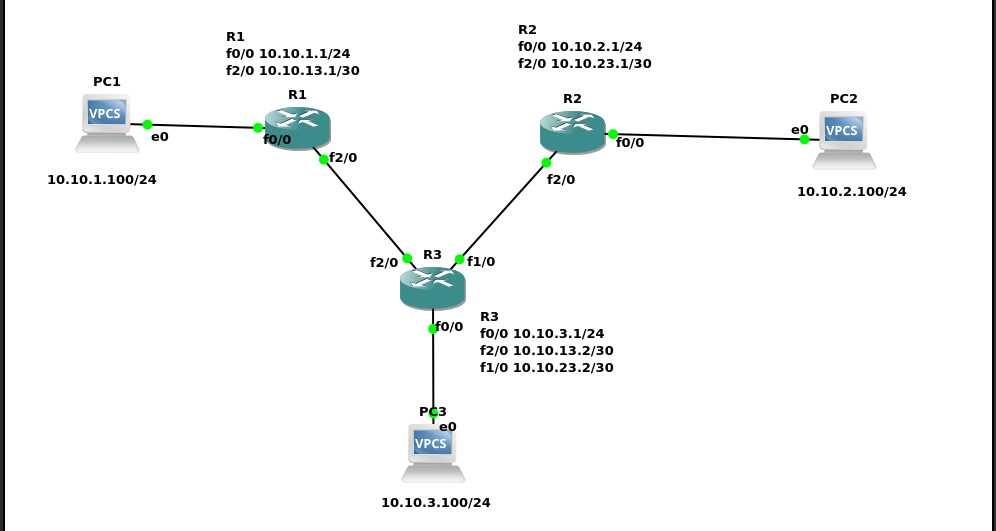
\includegraphics[scale=0.5]{imgs/1.png}
  \\\textit{Figura 1: Topología de la red utilizada}
\end{center}
\subsection{Archivos de configuración VPC}
\textit{Nota con fines de la imagen es necesario cambiar las VPCs por VMs ya que se hara uso del comando telnet para más adelante, solo se adapto esta parte por fines de que sea sencilla la configuración rápida de los dispositivos y se conozca al menos como se configuran.}
\subsubsection{VPC1}
\lstinputlisting[language=bash]{files/vpc1.cfg}
\subsubsection{VPC2}
\lstinputlisting[language=bash]{files/vpc2.cfg}
\subsubsection{VPC3}
\lstinputlisting[language=bash]{files/vpc3.cfg}
\subsection{Archivos de configuración Routers}
Para esto es posible solo copiar y pegar todo el archivo de configuración de acuerdo con el router y el archivo a utilizar directamente.
\subsubsection{Router 1}
\lstinputlisting[language=bash]{files/router1.cfg}
\clearpage
\subsubsection{Router 2}
\lstinputlisting[language=bash]{files/router2.cfg}
\subsubsection{Router 3}
\lstinputlisting[language=bash]{files/router3.cfg}
\subsection{Comandos}
Con estos archivos de configuración no solamente tendremos las interfaces de red ya configuradas, sino que ya tendremos el enrutamiento OSPF activido con su respectiva interfaz de loopback, de igual forma tendremos configuradas las politicas de QoS:
\begin{itemize}
  \item Asignación de tráfico ICMP con la precedencia de IP 1
  \item Asignación de tráfico HTTP con la precedencia de IP 3
  \item Asignación de tráfico OSPF con la precedencia de IP 7
  \item Control de tráfico ICMP a máximo 8Kbps
  \item Asignación de ancho de banda de 10Mbps para el tráfico HTTP
  \item Configuración de prioridad estricta para el tráfico de OSPF y asignación de 1Mbps de ancho de banda
\end{itemize}
Con esto ejecutara lo siguiente, de acuerdo al orden presentado y a los dispositivos previamente descritos.
\lstinputlisting[language=bash]{files/cmd.sh}
\textit{De acuerdo con lo anteriormente realizado se obtendra las siguientes capturas para el caso de policy-map de las interfaces de red de los router puede cambiar si es un caso automatico del duplex y otros parametros.}\\
Entonces si se ejecutan correctamente se obtendran los siguientes datos que se muestran en las caputras.
\begin{center}
  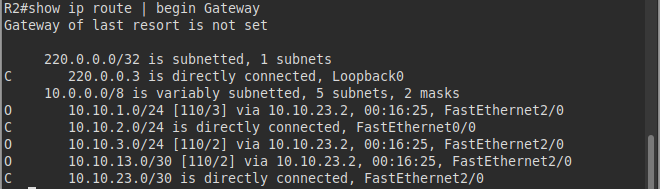
\includegraphics[scale=0.5]{imgs/2.png}\\
  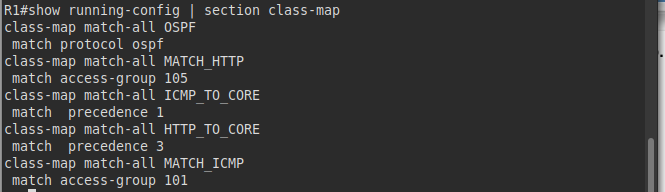
\includegraphics[scale=0.5]{imgs/3.png}\\
  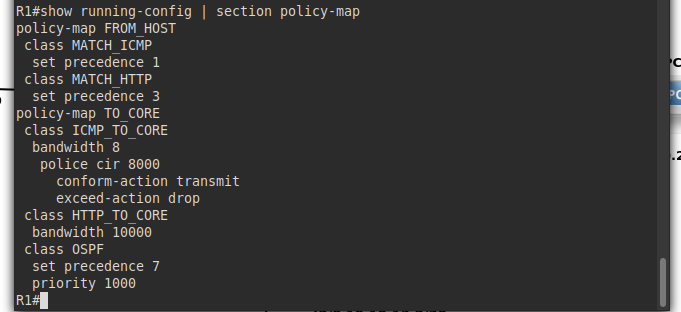
\includegraphics[scale=0.5]{imgs/4.png}\\
  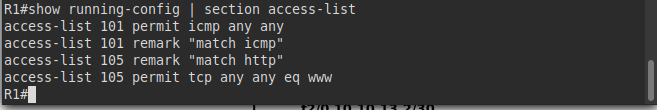
\includegraphics[scale=0.5]{imgs/5.png}\\
  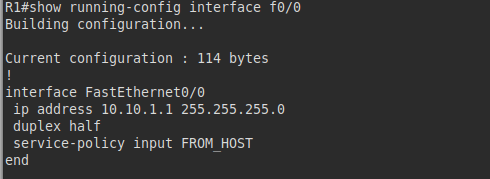
\includegraphics[scale=0.5]{imgs/6.png}\\
  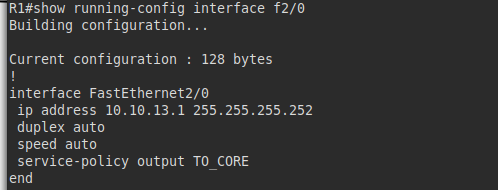
\includegraphics[scale=0.5]{imgs/7.png}\\
  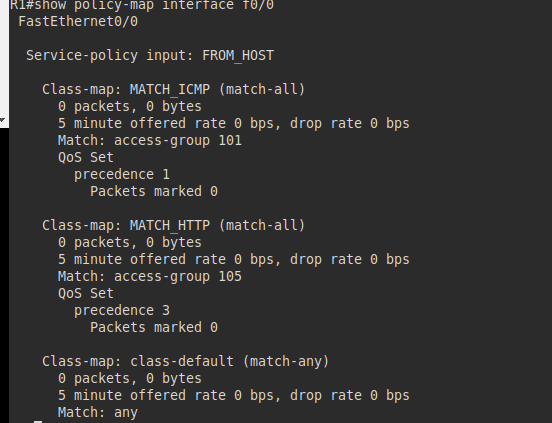
\includegraphics[scale=0.5]{imgs/8.png}\\
  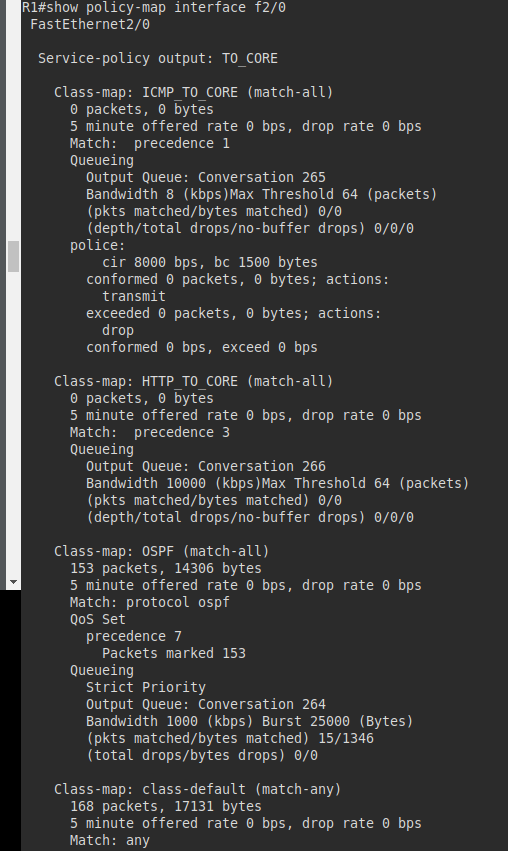
\includegraphics[scale=0.5]{imgs/9.png}
  \\\textit{Figuras 2-9: Ejecución de la primer serie de comandos}\\
  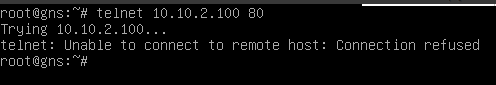
\includegraphics[scale=0.5]{imgs/10.png}
  \\\textit{Figuras 10: Ejecución del comando telnet para conexión al sever HTTP de la VPC2}\\
  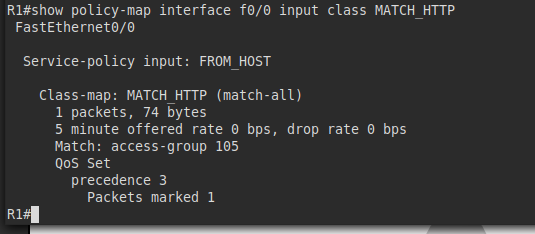
\includegraphics[scale=0.5]{imgs/11.png}\\
  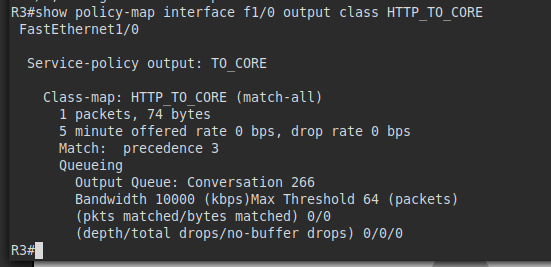
\includegraphics[scale=0.5]{imgs/12.png}
  \\\textit{Figuras 11-12: Verificación del trafico realizado a la regla HTTP de nuestra maquina virtual en los routers}\\
  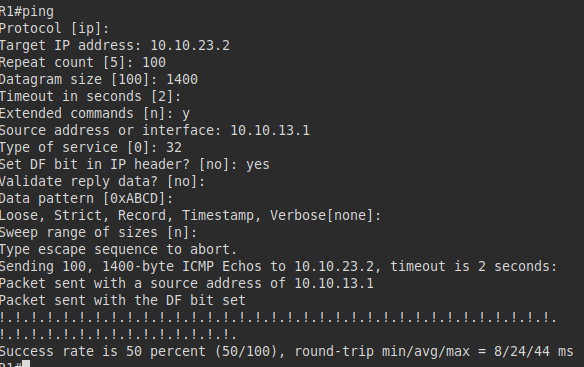
\includegraphics[scale=0.5]{imgs/13.png}\\
  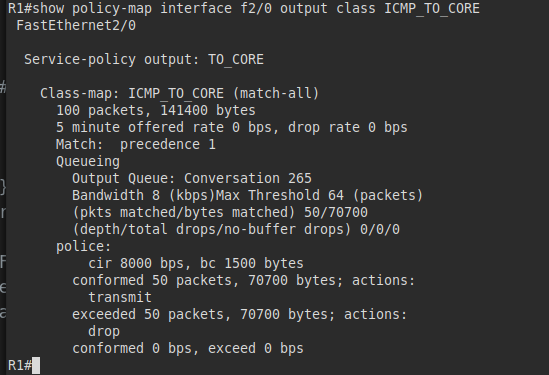
\includegraphics[scale=0.5]{imgs/14.png}\\
  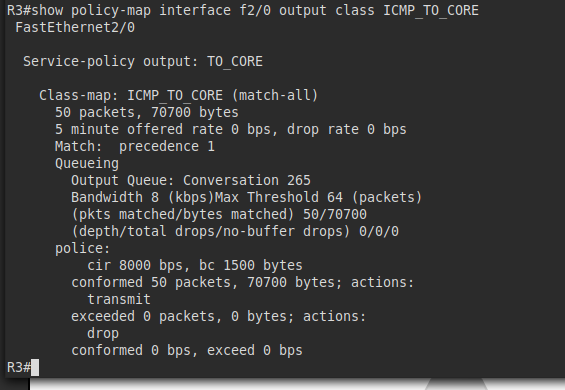
\includegraphics[scale=0.5]{imgs/15.png}
  \\\textit{Figuras 13-15: Verificación del trafico realizado a la regla ICMP de nuestro R1 hacia otra red exterior y el como esta solo envia el 50\% de los paquetes de acuerdo a nuestra configuración de QoS}
\end{center}
\end{document}
